% Status: Zweitprüfung
\chapter{Einführung} 
% TODO: Einführung 
\section{Unternehmensvorstellung} 
Eine Vorstellung des Unternehmens Unitedprint.
Geplanter Inhalt:
\begin{itemize}
    \item Unternehmensgeschichte
    \item Unitedprint ist ein Unternehmen, welches mehrere Webshops für den Vertrieb von Druckprodukten vertreibt. 
    \item Die Portale werde in allen europäische Ländern betrieben. 
    \item Eines der Portale ist das Portal \emph{easyprint.com} welches den FreeDesign-Editor integriert.
\end{itemize}

\section{Der FreeDesign-Editor}
\label{Der FreeDesign-Editor}
\subsection{Funktionsbeschreibung}
Der, durch Unitedprint bereitgestellte, Webshop \emph{easyprint.com} bietet Kunden die Möglichkeit Druckprodukt online zu gestaltet und im Anschluss zu bestellen. Für die Gestaltung der Produkte wurde unternehmenintern die Webanwendung \emph{FreeDesign} entwickelt, welche beständig gepflegt und weiterentwickelt wird. Die Anwendung ist eine Single-Page-Webanwendung, welche in der Programmiersprache TypeScript, sowie unter der Verwendung von \emph{ReactJS} und \emph{Redux} entwickelt wurde. 

Basierend auf Flanagan (\citeyear[S. 497]{Flanagan2006}) wird als Single-Page-Webanwendung ein Webanwendung bezeichnet die auf der Ajax-Technologie basiert und ihre Inhalt per JavaScript aktualisiert und nicht durch das neu Laden der Anwendung. 

Mit hilfe des Editor kann eine große Vielzahl von Druckprodukten gestaltet werden, wobei das Portfolio verschiedenste Produktgruppen, wie Bürozubehör, Textilien oder Werbematerialien, abdeckt. Zur Gestaltung eines Designs bietet der Editor die Möglichkeit der Nutzung eigener Text und Bilder sowie das Verwenden verschiedenster geometrischer Formen. Alle Element können umfangreich geometrisch und grafische bearbeitet werden. Um einen optimalen Gestaltungsprozess zu ermöglichen, kann die Produktdarstell auch wärend der Gestaltung vergrößert, verschoben oder rotiert werden. Weiterhin stehen auch Hilfwerkzeuge wie Lineal oder Hilflinien zur Verfügung. 

Die Nutzer haben auch die Möglichkeit Designs als Entwürfe zu speicheren und zu einem späteren Zeitpunkt zu öffnen.

\begin{figure}[H]
    \centering
    \efbox{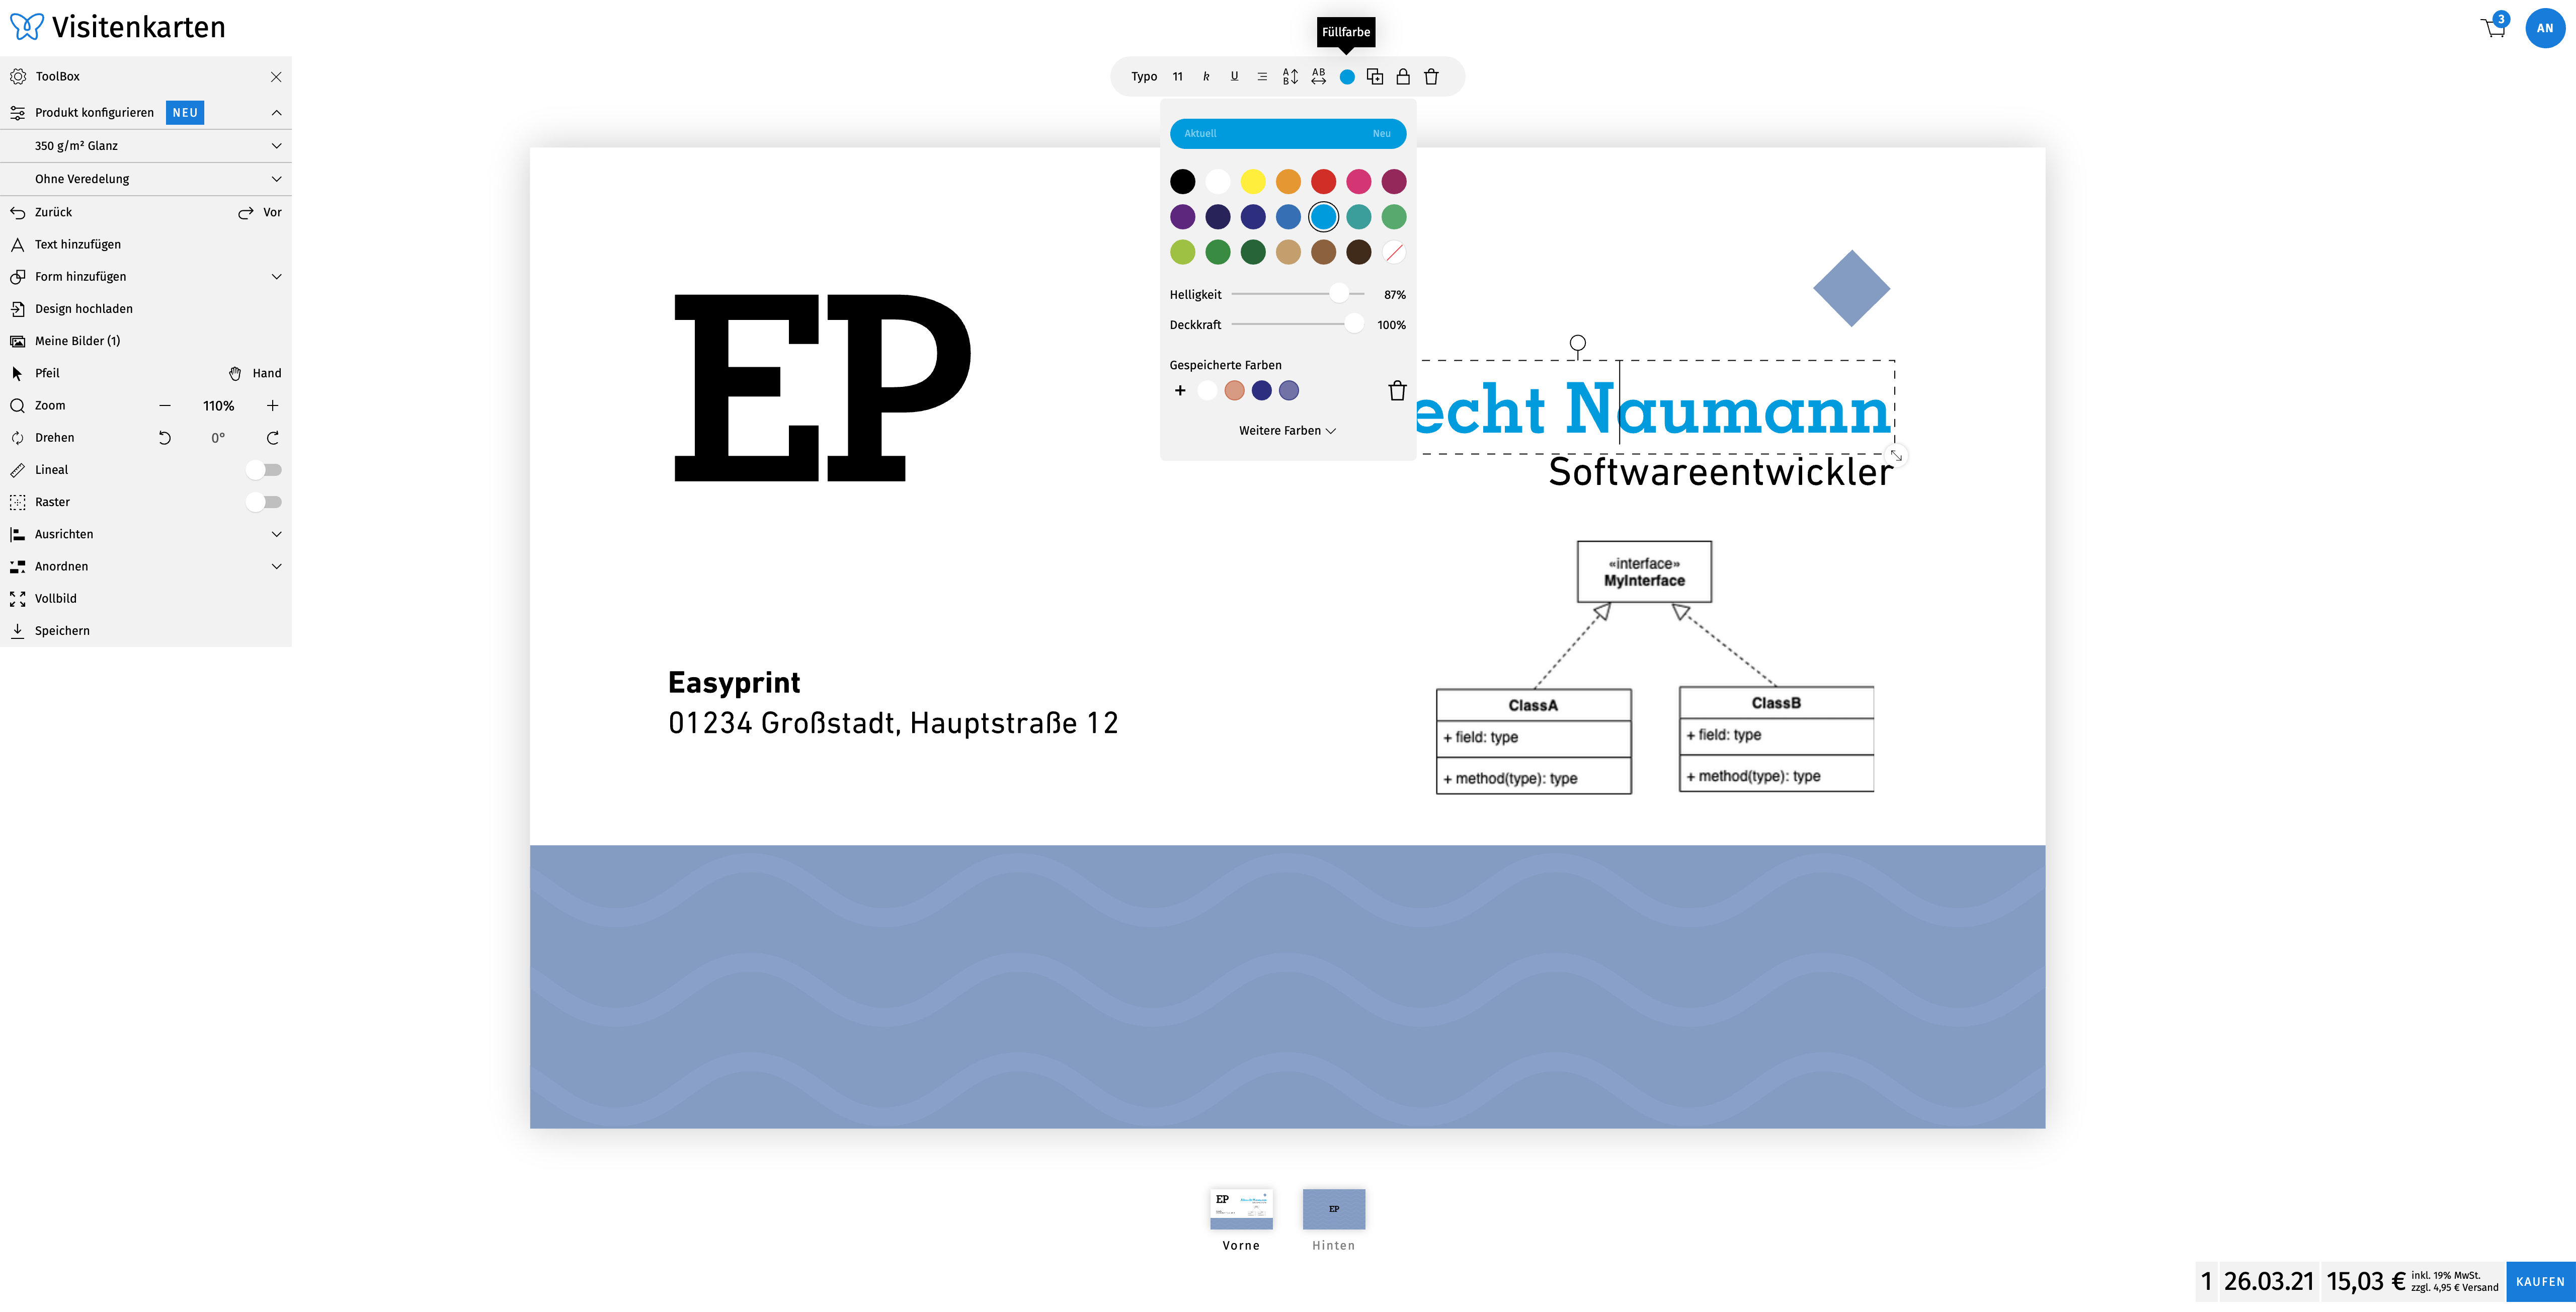
\includegraphics[width=.98\textwidth]{chapter/freedesign/Screenshot-Freedesign.png}}
    \caption{Ein Bildschirmfoto des FreeDesign-Editor}
    \label{fig:Der FreeDesign-Editor}
\end{figure}

\subsection{Designvorlagen}

\begin{figure}[H]
    \centering
    \efbox{\includegraphics[width=.98\textwidth]{chapter/freedesign/Screenshot-Designseite.png}}
    \caption{Ein Bildschirmfoto der Designübersichtseite für Visitenkarten}
    \label{fig:Designuebersichtseite}
\end{figure}

\begin{figure}[H]
    \centering
    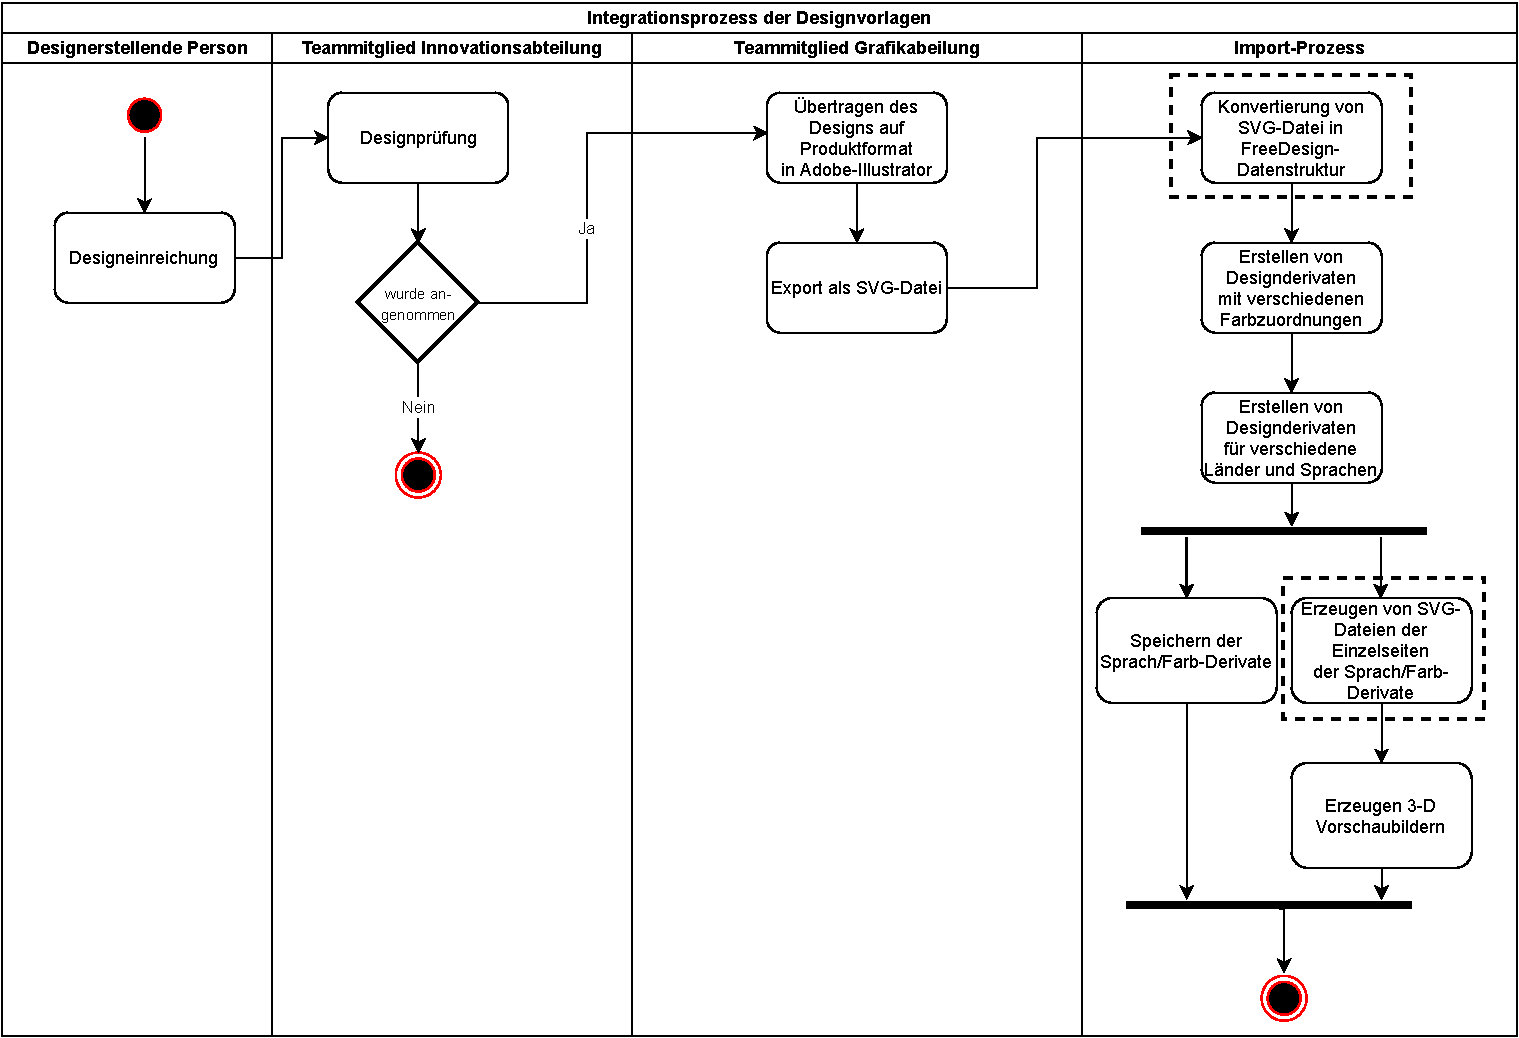
\includegraphics[width=.98\textwidth]{diagrams/Freedesign-Vorlagenerstellung.pdf}
\caption{Prozessbeschreibung der Vorlagenerstellung}
\label{fig:Vorlagenimport}
\end{figure}

\subsection{Bestellablauf}
%TODO: => Auf Team eingehen



% \subsubsection{Externe Schnittstellen}
Der FreeDesign-Editor kommuniziert über folgende vier Schnittstellen:
\begin{itemize}
	\item Über eine grafische Oberfläche wird der Editor vom Nutzer bedient und die Anwendung reagiert sowohl auf Mauseingaben als auch auf Tastatureingaben. 
	\item Zur Kommunikation mit Unitedprint-Backend wird eine REST-API genutzt. 
	\item Der Editor wird mit einer Reihen von URL-Parametern aufgerufen, die steuern, welche Produkt-Konfiguration von der Anwendung geladen wird. Über die URL-Parameter kann auch das Laden von Designvorlagen oder Kundendesign gesteuert, sowie weiter Funktionalitäten des Editors aktiviert werden. 
	Innerhalb des Editor besteht auch die Möglichkeit das Produkt zu ändern, worauf hin die URL sich aktualisiert.
	\item Ein Browser-Cookie wird vorwiegend zur Nutzer-Authentifizierung genutzt. 
\end{itemize}

Browser bieten die Möglichkeiten Daten in einem Local-Storage-Object oder einem Session-Storage-Object Daten zu speichern. \autocite{Mozilla:Storage}
Die werden jedoch aktuell von der Anwendung nicht genutzt. 

% TODO: Es fehlt das Clipboard

\begin{figure}[H]
    \centering
    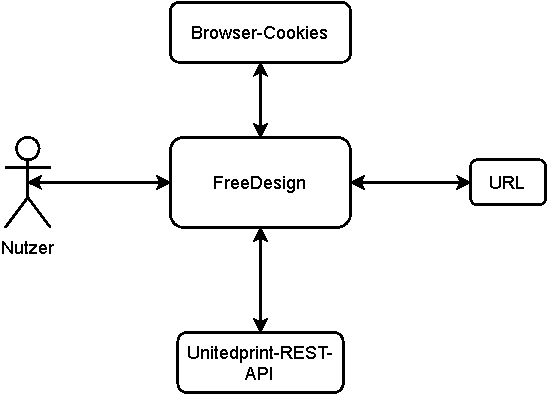
\includegraphics{diagrams/Ist-Architektur/Freedesign_Interaktion.pdf}
     \caption{Externe Schnittstellen}
     \label{fig:Externe_Schnittstellen}
  \end{figure}
  

\section{Problemstellung}
Als Anfang 2018 die Entwicklung der aktuellen FreeDesign-Anwendung begonnen wurde, hatte das Team nur wenig Erfahrung im Entwickeln von ReactJS-Anwendungen. Des Weiteren wurde die Anwendung unter einem hohen zeitlichen Druck entwickelt.
Dadurch sind eine Reihe von technischen Schulden entstanden. Eine der Hauptschulden ist eine fehlende Definition der Quelltext-Architektur. Durch die Verwendung von ReactJS und Redux wird zwar bereits eine gewisse Architektur vorgeben, diese bezieht sie jedoch auf die Strukturierung der grafischen Oberfläche. Für die Domain-Logik wurde jedoch keine spezifische Architektur festgelegt, was die Pflege und Weiterentwicklung der Anwendung, erschweren kann.
Die aktuelle Architektur weist derzeit folgende offensichtliche Schwächen auf:
\begin{itemize}
  \item Die Architektur ist nicht dokumentiert.
  \item Der Quelltext für die grafische Oberfläche und für die Domain-Logik sind mitunter viel
  zu eng gekoppelt, was den Austausch und die Aktualisierung von JavaScript-
  Bibliotheken erschwert.
  \item Durch die zuvor genannte enge Kopplung ist es für einige Teile des Quelltextes
  schwer Unit-Tests zu erstellen bzw. zu pflegen.
  \item Einige Teile des Quelltextes weisen Anzeichen von Anti-Patterns auf.
\end{itemize}
Da die Anwendung einer permanenten Weiterentwicklung unterliegt, ist es wichtig die Software in eine geeignetere Architektur zur überführen. Weiterhin entwickelt sich die Webtechnologie mit großer Geschwindigkeit weiter. An dieser Stelle ist eine Architektur notwendig, die eine effiziente Pflege ermöglicht.

\section{Ziel der Diplomarbeit}
Das Ziel der Diplomarbeit ist die Ausarbeitung eines Vorgehens zur Überführung einer Ist-Architektur einer, in TypeScript implementierten, ReactJS-Anwendung in eine Soll-Architektur. Um eine hohe Akzeptanz einer solcher Maßnahme zu erreichen, ist eine Rahmenbedingung, dass die Überführung schrittweise geschieht und die Weiterentwicklungsarbeit der ReactJS-Anwendung begleitet.
% TODO: noch mehr einschränken => statische Ist-Architektur